\documentclass[tikz]{standalone}
\usepackage{amsmath}
\definecolor{bg}{HTML}{171D2B}
\definecolor{acc}{HTML}{F7B538}
\definecolor{wht}{HTML}{FFFFFF}
\begin{document}
\pagecolor{bg}
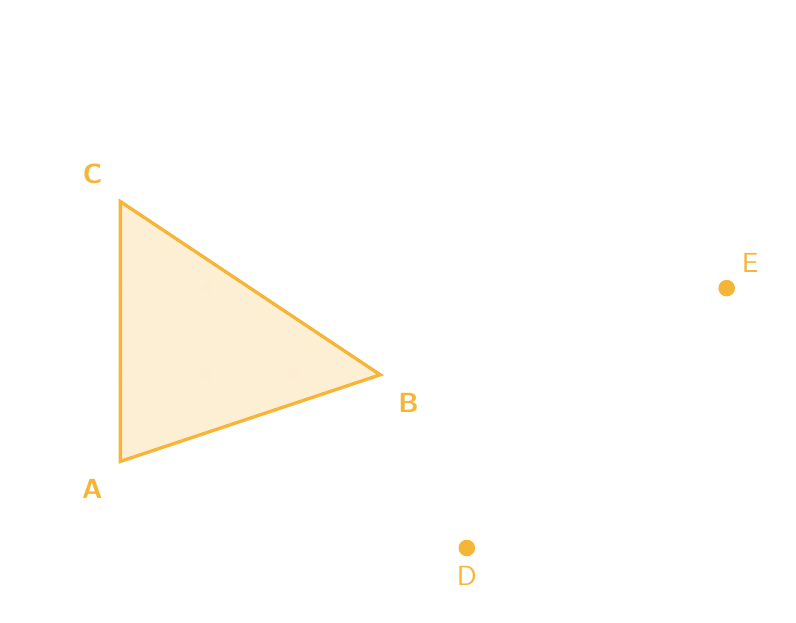
\begin{tikzpicture}[
  every node/.style={text=wht, font=\sffamily},
  main/.style={draw=acc, very thick},
  kotak/.style={draw=wht!50, dashed},
]
% papan titik 9x6 (baris 0..5, kolom 0..8), jarak antarpaku 1.1cm
\def\cols{8}\def\rows{5}
\foreach \i in {0,...,\cols} \foreach \j in {0,...,\rows}
  \fill[wht!60] (\i*1.1,\j*1.1) circle (2.2pt);

% karet band 1: segitiga A(1,1), B(4,2), C(1,4)
\coordinate (A) at (1.1,1.1);
\coordinate (B) at (4.4,2.2);
\coordinate (C) at (1.1,4.4);
\fill[acc, fill opacity=0.22] (A) -- (B) -- (C) -- cycle;
\draw[main] (A) -- (B) -- (C) -- cycle;
\foreach \P/\pos/\nama in {A/below left/A, B/below right/B, C/above left/C}
  \node[\pos=3pt, font=\sffamily\bfseries, text=acc] at (\P) {\nama};

% karet band 2: garis D(5,0) - E(8,3)
\coordinate (D) at (5.5,0);
\coordinate (E) at (8.8,3.3);
\draw[main, wht, very thick] (D) -- (E);
\fill[acc] (D) circle (3pt);
\fill[acc] (E) circle (3pt);
\node[below=3pt, text=acc] at (D) {D};
\node[above right=2pt, text=acc] at (E) {E};

\node[above=14pt, font=\sffamily\large\bfseries, text=wht] at (4.4,5.5) {Papan Geoboard};
\end{tikzpicture}
\end{document}
